%%%%%%%%%%%%%%%
%							TEST MODEL 
%%%%%%%%%%%%%%%

\subsection{Project Test Model} \label{section:project-model}

%New Paragraph
This section outlines the test model that was created after the draft model stage, QUT data access and initial photovoltaic systems analysis. In order to create the test model of a ``real-world" Brisbane based commercial building to structure the analysis around, the QUT schematics and personal experience within Brisbane's built environment were integral. 

\subsubsection{Lighting Loads}

%New Paragraph
To calculate approximate lighting loads to be expected for a floor, level 7 of QUT P\,Block was marked up to count the number of luminaires installed. A full floor plan is shown in Appendix \ref{appendix:qut_lvl6_markup} but an image export is below in Figure \ref{fig:qut-lvl6-lighting-markup}.      

\begin{figure}[H]
	\hfill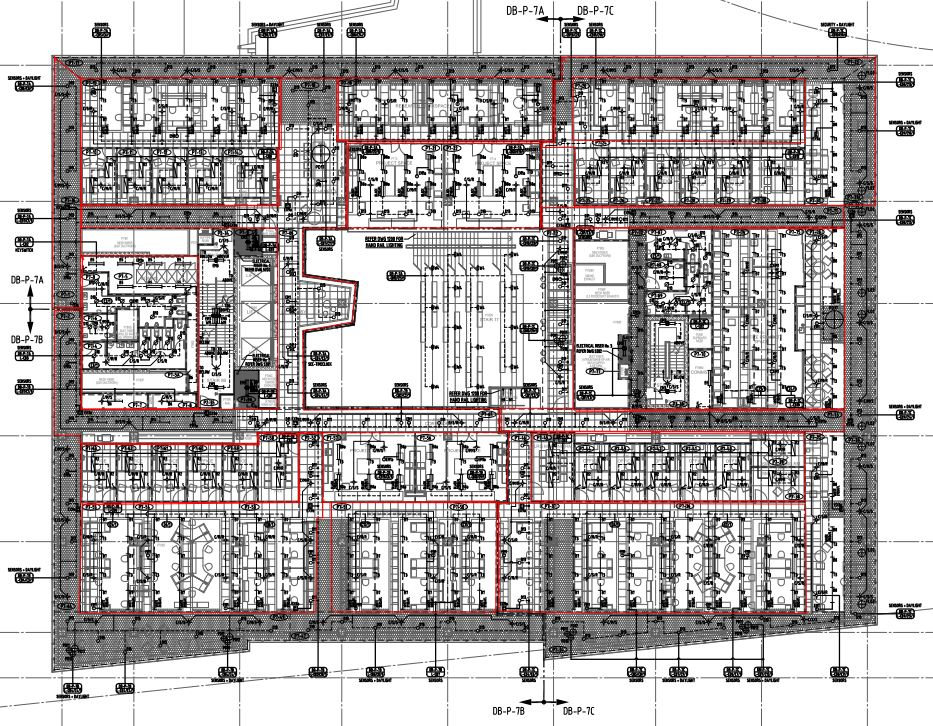
\includegraphics[width = 150mm]{images/project-model/qut-lvl7-lighting-markup}\hspace*{\fill}
	\caption{QUT: P Block Level 6 Lighting Markup} 
	\label{fig:qut-lvl6-lighting-markup}
\end{figure}

%New Paragraph
Table \ref{table:QUTlvl7-count} below outlines the counts from the markup. These were then used to calculate total loads for the floor plan. With these values, a test model can be based with an approximate light load that can be separated over dedicated DC distribution boards over the floor once further calculations and photovoltaics layouts are designed. This model will be utilised in Section \ref{section:project-questions} for deep analysis and simulation. This is the reasoning behind utilising the QUT provided floor plans to attempt to create an accurate ``real world" example of DC distribution implementation.     

\begin{table}[!ht]
	\centering
	\renewcommand{\arraystretch}{2}
	\begin{tabular}{|c|c|c|c|c|}
		\hline
		\textbf{Fitting} & \textbf{Wattage (W)} & \textbf{Voltage (V)} & \textbf{Count} & \textbf{Demand (A)} \\ \hline
		2x18W Fluorescent & 18.0 & 24.0 & 220 & 0.75 \& 165 \\ \hline
		2x28W Fluorescent & 28.0 & 24.0 & 448 & 1.17 \& 520 \\ \hline
	\end{tabular}

	\caption{QUT: P Block Level 7 Lighting Count and Calculations}
	\label{table:QUTlvl7-count}
\end{table}

\subsubsection{Floor Size}

%New Paragraph
The same floor plan layout was loaded into AutoCad to calculate the area and average room size. The entire floor plan was measure to be approximate 65\,m by 47\,m providing an area of approximately 3000\,\si{m^2}. The average office size of 22\,\si{m^2}. 

\subsubsection{Photovoltaic Modules}

%New Paragraph
This information is elaborated on further in Section \ref{section:PV-panels} however to briefly preface, the test model will be based on utilising the average photovoltaic module of 265\,W of assumed size 1600\,mm by 1000\,mm by 35\,mm. This value will be used in analysisng PV quantities with available spacings as well as power production simulation with System Advisor Model. 

\subsubsection{Electrical Infrastructure}

%New Paragraph
The assumption for this project is that separate DC electrical infrastructure will be installed to power the chosen devices. At this stage, devices cannot be selected because loads have to be analysed first after photovoltaic modelling. Ideally, reputable brands for electrical equipment such as Eaton or NHP will be selected with preference to affordable but safe models. Eaton products are generally more affordable and will likely be chosen for the switchboards and circuit breakers. Additionally, it is generally far easier to alter settings to remove faults when the same manufacturer is used for the complete circuits.  
       
  
 